\documentclass[11pt]{article}

\usepackage{times}
\usepackage{epsf}
\usepackage{epsfig}
\usepackage{amsmath, alltt, amssymb, xspace}
\usepackage{wrapfig}
\usepackage{fancyhdr}
\usepackage{url}
\usepackage{verbatim}
\usepackage{fancyvrb}

\usepackage{subfigure}
\usepackage{cite}
%\usepackage{cases}
%\usepackage{ltexpprt}
%\usepackage{verbatim}

%\topmargin      -0.70in  % distance to headers
%\headheight     0.2in   % height of header box
%\headsep        0.4in   % distance to top line
%\footskip       0.3in   % distance from bottom line

% Horizontal alignment
\topmargin      -0.50in  % distance to headers
\oddsidemargin  0.0in
\evensidemargin 0.0in
\textwidth      6.5in
\textheight     8.9in 


%\centerfigcaptionstrue

%\def\baselinestretch{0.95}


\newcommand\discuss[1]{\{\textbf{Discuss:} \textit{#1}\}}
%\newcommand\todo[1]{\vspace{0.1in}\{\textbf{Todo:} \textit{#1}\}\vspace{0.1in}}
\newtheorem{problem}{Problem}[section]
%\newtheorem{theorem}{Theorem}
%\newtheorem{fact}{Fact}
\newtheorem{define}{Definition}[section]
%\newtheorem{analysis}{Analysis}
\newcommand\vspacenoindent{\vspace{0.1in} \noindent}

%\newenvironment{proof}{\noindent {\bf Proof}.}{\hspace*{\fill}~\mbox{\rule[0pt]{1.3ex}{1.3ex}}}
%\newcommand\todo[1]{\vspace{0.1in}\{\textbf{Todo:} \textit{#1}\}\vspace{0.1in}}

%\newcommand\reducespace{\vspace{-0.1in}}
% reduce the space between lines
%\def\baselinestretch{0.95}

\newcommand{\fixmefn}[1]{ \footnote{\sf\ \ \fbox{FIXME} #1} }
\newcommand{\todo}[1]{
\vspace{0.1in}
\fbox{\parbox{6in}{TODO: #1}}
\vspace{0.1in}
}

\newcommand{\mybox}[1]{
\vspace{0.2in}
\noindent
\fbox{\parbox{6.5in}{#1}}
\vspace{0.1in}
}


\newcounter{question}
\setcounter{question}{1}

\newcommand{\myquestion} {{\vspace{0.1in} \noindent \bf Question \arabic{question}:} \addtocounter{question}{1} \,}

\newcommand{\myproblem} {{\noindent \bf Problem \arabic{question}:} \addtocounter{question}{1} \,}


\newcommand{\copyrightnoticeA}[1]{
\vspace{0.1in}
\fbox{\parbox{6in}{\small Copyright \copyright\ 2006 - 2014\ \ Wenliang Du, Syracuse University.\\ 
      The development of this document is partially funded by 
      the National Science Foundation's Course, Curriculum, and Laboratory 
      Improvement (CCLI) program under Award No. 0618680 and 0231122. 
      Permission is granted to copy, distribute and/or modify this document
      under the terms of the GNU Free Documentation License, Version 1.2
      or any later version published by the Free Software Foundation.
      A copy of the license can be found at http://www.gnu.org/licenses/fdl.html.}}
\vspace{0.1in}
}


\newcommand{\copyrightnotice}[1]{
\vspace{0.1in}
\fbox{\parbox{6in}{\small Copyright \copyright\ 2006 - 2014\ \ Wenliang Du, Syracuse University.\\
      The development of this document is/was funded by three grants from
      the US National Science Foundation: Awards No. 0231122 and 0618680 from
      TUES/CCLI and  Award No. 1017771 from Trustworthy Computing.
      This lab was imported into the Labtainer framework by the Naval Postgraduate 
      School, Center for Cybersecurity and Cyber Operations under National Science 
      Foundation Award No. 1438893.
      Permission is granted to copy, distribute and/or modify this document
      under the terms of the GNU Free Documentation License, Version 1.2
      or any later version published by the Free Software Foundation.
      A copy of the license can be found at http://www.gnu.org/licenses/fdl.html.}}
\vspace{0.1in}
}

\newcommand{\copyrightnoticeB}[1]{
\vspace{0.1in}
\fbox{\parbox{6in}{\small Copyright \copyright\ 2006 - 2014\ \ Wenliang Du, Syracuse University.\\
      The development of this document is/was funded by the following grants from
      the US National Science Foundation: No. 0231122, 0618680, and 1303306.
      Permission is granted to copy, distribute and/or modify this document
      under the terms of the GNU Free Documentation License, Version 1.2
      or any later version published by the Free Software Foundation.
      A copy of the license can be found at http://www.gnu.org/licenses/fdl.html.}}
\vspace{0.1in}
}


\newcommand{\nocopyrightnotice}[1]{
\vspace{0.1in}
\fbox{\parbox{6in}{\small  
      The development of this document is funded by 
      the National Science Foundation's Course, Curriculum, and Laboratory 
      Improvement (CCLI) program under Award No. 0618680 and 0231122. 
      Permission is granted to copy, distribute and/or modify this document.
      }}
\vspace{0.1in}
}

\newcommand{\idea}[1]{
\vspace{0.1in}
{\sf IDEA:\ \ \fbox{\parbox{5in}{#1}}}
\vspace{0.1in}
}

\newcommand{\questionblock}[1]{
\vspace{0.1in}
\fbox{\parbox{6in}{#1}}
\vspace{0.1in}
}


\newcommand{\minix}{{\tt Minix}\xspace}
\newcommand{\unix}{{\tt Unix}\xspace}
\newcommand{\linux}{{\tt Linux}\xspace}
\newcommand{\ubuntu}{{\tt Ubuntu}\xspace}
\newcommand{\selinux}{{\tt SELinux}\xspace}
\newcommand{\freebsd}{{\tt FreeBSD}\xspace}
\newcommand{\solaris}{{\tt Solaris}\xspace}
\newcommand{\windowsnt}{{\tt Windows NT}\xspace}
\newcommand{\setuid}{{\tt Set-UID}\xspace}
%\newcommand{\smx}{{\tt Smx}\xspace}
\newcommand{\smx}{{\tt Minix}\xspace}
\newcommand{\relay}{{\tt relay}\xspace}
\newcommand{\isys}{{\tt iSYS}\xspace}
\newcommand{\ilan}{{\tt iLAN}\xspace}
\newcommand{\iSYS}{{\tt iSYS}\xspace}
\newcommand{\iLAN}{{\tt iLAN}\xspace}
\newcommand{\iLANs}{{\tt iLAN}s\xspace}
\newcommand{\bochs}{{\tt Bochs}\xspace}

\newcommand\FF{{\mathcal{F}}}

\newcommand{\argmax}[1]{
\begin{minipage}[t]{1.25cm}\parskip-1ex\begin{center}
argmax
#1
\end{center}\end{minipage}
\;
}

\newcommand{\bm}{\boldmath}
\newcommand  {\bx}    {\mbox{\boldmath $x$}}
\newcommand  {\by}    {\mbox{\boldmath $y$}}
\newcommand  {\br}    {\mbox{\boldmath $r$}}


%\pagestyle{fancyplain}
%\lhead[\thepage]{\thesection}      % Note the different brackets!
%\rhead[\thesection]{SEED Laboratories}
%\lfoot[\fancyplain{}{}]{Syracuse University} 
%\cfoot[\fancyplain{}{}]{\thepage} 

\newcommand{\tstamp}{\today}   
%\lhead[\fancyplain{}{\thepage}]         {\fancyplain{}{\rightmark}}
%\chead[\fancyplain{}{}]                 {\fancyplain{}{}}
%\rhead[\fancyplain{}{\rightmark}]       {\fancyplain{}{\thepage}}
%\lfoot[\fancyplain{}{}]                 {\fancyplain{\tstamp}{\tstamp}}
%\cfoot[\fancyplain{\thepage}{}]         {\fancyplain{\thepage}{}}
%\rfoot[\fancyplain{\tstamp} {\tstamp}]  {\fancyplain{}{}}

\pagestyle{fancy}
%\lhead{\bfseries Computer Security Course Project}
\lhead{\bfseries SEED Labs}
\chead{}
\rhead{\small \thepage}
\lfoot{}
\cfoot{}
\rfoot{}

\usepackage{listings}
\usepackage{color}

\definecolor{dkgreen}{rgb}{0,0.6,0}
\definecolor{gray}{rgb}{0.5,0.5,0.5}
\definecolor{mauve}{rgb}{0.58,0,0.82}

\lstset{frame=tb,
  language=C,
  aboveskip=3mm,
  belowskip=3mm,
  showstringspaces=false,
  columns=flexible,
  basicstyle={\small\ttfamily},
  numbers=none,
  numberstyle=\tiny\color{gray},
  keywordstyle=\color{blue},
  commentstyle=\color{dkgreen},
  stringstyle=\color{mauve},
  breaklines=true,
  breakatwhitespace=true,
  tabsize=3
}



\begin{document}

\begin{center}
{\LARGE Radius Authentication Service}
\vspace{0.1in}\\
\end{center}

\copyrightnotice

\section{Overview}
In this lab you will configure a Radius server to handle authentication
services for a network device that is already configured to use Radius-based
authentication.  The Radius server is pre-configured to support an existing
network device.  You are simply required to add the second device.
In this lab, the Radius protocol is configured to use a shared secret known
to the Radius server, and the devices that authenticate via that server.
The shared secret for both devices is the same.

You are encouraged to use Wireshark within the lab to observe the Radius
protocol exchanges.

Radius provides Authentication, Authorization and Accounting (AAA) functions.  The protocol is rich and 
supports many options.  Details of the protocol can be found at: \url{https://tools.ietf.org/html/rfc2865}.
While Radius orignally was used to manage AAA for dial-up facilities, it is broadly used for networked devices,
including embedded systems such as smart power supplies.

This lab will touch on the basics of using Radius for centralized authentication, and it will demonstrate
and example of Radius accounting. The lab uses the
FreeRADIUS product, which is detailed here \url{https://networkradius.com/doc/3.0.10/introduction/RADIUS.html}

\subsection {Background}
The student is expect to have separately learned about the basic elements of authentication
and the Radius protocol.

The student is expected to have at least a basic understanding of the Linux command line,
the basics of the file system, and the ability to edit a file.  The student should have
knowledge of the use of Wireshark, e.g., see the ``wireshark-intro'' lab.

\section{Lab Environment}
This lab runs in the Labtainer framework,
available at http://nps.edu/web/c3o/labtainers.
That site includes links to a pre-built virtual machine
that has Labtainers installed, however Labtainers can
be run on any Linux host that supports Docker containers.

From your labtainer-student directory start the lab using:
\begin{verbatim}
    labtainer radius
\end{verbatim}
\noindent A link to this lab manual will be displayed.  

\section{Network Configuration}
This lab includes two simulated power distribution control devices that
are configured to authenticate users via the Radius protocol.  In the jargon
of Radius, the control devices are Network Access Server (NAS), i.e., they
provide access to the power distirbution functions in our exercise. There
are also two client computers from which users are expected to administer
the control devices.  
And the network includes a Radius server.  NOTE: the control devices
do not have virtual terminals connected to them, so the only way to 
access them is through the client computers.  The network is
illustrated in Figure~\ref{fig:topology}.
When the lab starts, you will get three terminals, one connected to each
of the client computers and one connected to the Radius server.

The host names of each component are per the diagram.  The /etc/hosts files
allow use of these host names instead of explicit ip addresses.

\begin{figure}[H]
\begin{center}
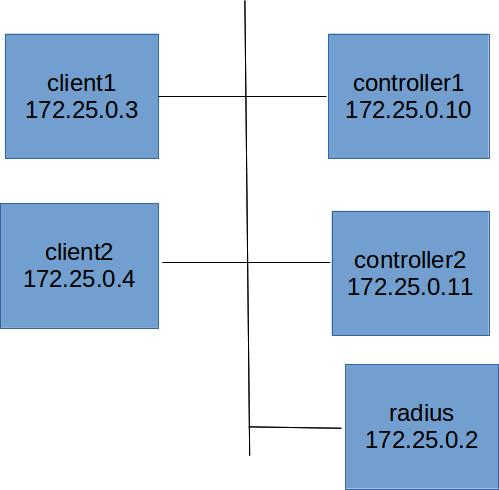
\includegraphics [width=0.8\textwidth]{radius.jpg}
\end{center}
\caption{Network topology for the Radius lab}
\label{fig:topology}
\end{figure}

\section{Lab Tasks}
\subsection{Explore}
Start wireshark on the radius server:
\begin{verbatim}
   wireshark &
\end{verbatim}
\noindent and select the eth0 interface and start capturing data.

Then start the radius service in foreground and debug mode:
\begin{verbatim}
    radiusd -fX
\end{verbatim}

View the {\tt control\_admin} script on client1.  Note it simply uses {\tt ssh} to execute a program
on a named remote controller.  Typically, ssh requires a password or key pairs.  The control devices
lack password or key management.  Instead, control devices are configured to defer ssh daemon authentication decisions to
the Radius server.

On client1, connect to controller1:
\begin{verbatim}
    ./control_admin controller1
\end{verbatim}
\noindent When prompted, provide {\tt hardcoded\_password} as the password.
\footnote{If the control\_admin program
repeatedly informs you that the password is not correct, that may be
due to the radius service not running.}
Observe the traffic in wireshark. 

Then use {\tt exit} to exit from controller1.  And now try to access
controller2, again using a password of: {\tt hardcoded\_password}
\begin{verbatim}
    ./control_admin controller2
\end{verbatim}
\noindent What do you observe at the radius service?  And in wireshark?

\subsection{Configure radius for controller2}
The controller2 device has been pre-configured to use your Radius server for 
authentication of users.  That means it has the shared secret used by Radius
to encrypt user passwords, and it knows the IP address of the radius server.
However, the Radius server is not configured to serve controller2.  You must
change the Radius server configuration to recognize controller2.
Use Ctrl-c at the radius server to stop the service.
Edit the {\tt /etc/raddb/clients.conf} file to allow controller2 to authenticate
via the radius service, and then restart the radius service.

Try again to access controller2 from one of the clients.

\subsection{Change the cadmin password}
Stop the radius service and edit the {\tt /etc/raddb/users} file to change the 
password of the cadmin user to something other than {\tt hardcoded\_password}.  Then test your abilty
use the control\_admin  utility to access the controllers with the new password.

\subsection{Accounting}
On the radius server, view the directories and files beneath the {\tt /var/log/radius} directory.
Note how each NAS has its own accounting file.  

\section{Submission}
After finishing the lab, go to the terminal on your Linux system that was used to start the lab and type:
\begin{verbatim}
    stoplab 
\end{verbatim}
When you stop the lab, the system will display a path to the zipped lab results on your Linux system.  Provide that file to 
your instructor, e.g., via the Sakai site.

\end{document}
